\section{Auswertung}
\label{sec:Auswertung}

\subsection{Lange Spule}

Die lange Spule wird so an eine Messvorrichtung angebracht, dass das linke Ende der Spule
bei $x=0$ ist. Die Spule wird bei beliebiger Spannung mit einem Strom von 1 A betrieben. Mithilfe einer
logitudinalen Hall-Sonde werden nun 10 Messwerte für das Magnetfeld innehalb der Spule aufgenommen. \\
Die lange Spule hat eine Windungszahl von $n=300$ und einen mittlerer Spulendurchmesser von $d = 41 \, \unit{\mm}$.
Da während des Versuchs die Länge der Spule nicht gemessen wurde, wird diese anhand von den Messwerten
auf 15 cm geschätzt. Die Messwerte der Versuchsreihe finden sich in \autoref{tab:Spule}.

\begin{table}
  \centering
  \caption{Messwerte des Magnetfelds der langen Spule.}
  \label{tab:Spule}
  \begin{tabular}{c c}
    \toprule
    $B/\unit{\tesla} \cdot 10^{-3}$ & $x/\unit{\cm}$ \\
    \midrule
     -0,9 & 1 \\
     -1,3 & 2 \\
     -1,8 & 3 \\
     -2,1 & 4 \\
     -2,2 & 5 \\
     -2,3 & 6 \\
     -2,3 & 7 \\
     -2,4 & 8 \\
     -2,4 & 9 \\
     -2,4 & 10 \\
    \bottomrule
  \end{tabular}
\end{table}

\begin{figure}
  \centering
  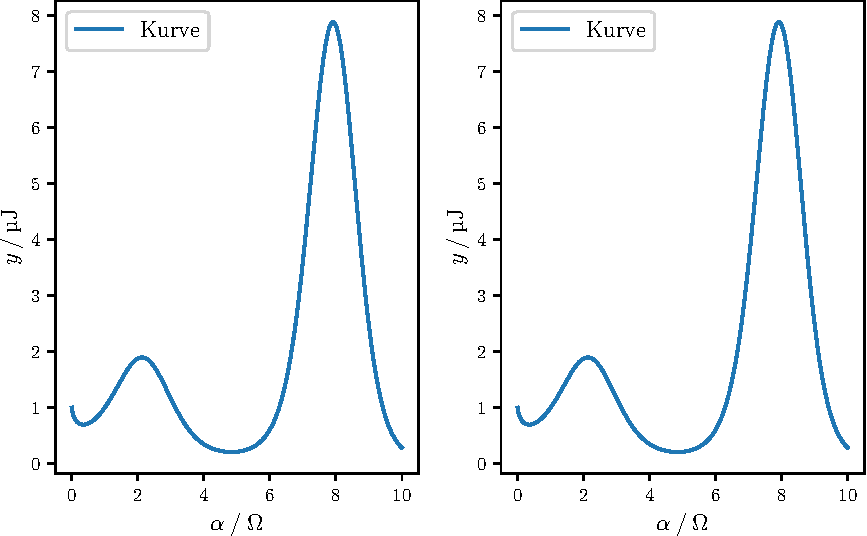
\includegraphics{plot.pdf}
  \caption{Magnetfeldstärke bei verschiedenen Abständen $x$ zum Spulenrand}
  \label{fig:Spule}
\end{figure}

In \autoref{fig:Spule} sind die Messwerte aus \autoref{tab:Spule} mit roten Kreuzen dargestellt. Auf der
x-Achse wird der Abstand zum linken Spulenrand aufgetragen und auf der y-Achse die gemessenen Magnetfeldstärken
in mT. \\
In einer Spule lässt sich ein relativ homogenes Feld herstellen, welches sich wie in \autoref{eqn:nSpule}
verhält. Anhand dieser Gleichung wird die blaue Theoriekurve zu den gegebenen Werten geplottet.\\
Da der Unterschied zu den Messwerten deutlich sichtbar ist, wird ebenfalls eine optimierte Kurve geplottet,
wo der Strom $I$ und die Windungszahl $n$ so verändert wird, dass die Amplitude der Kurve sich an
die Messwerte angleicht. Zwischen den Messwerten und der Theoriekurve besteht eine prozentuale Abweichung 
von 283 \%. \\

\subsection{Helmholtz-Spulenpaar}

Bei diesem Versuch wird ein Helmholtz-Spulenpaar verwendet. Dieses wird mit drei verschiedenen Abständen 
zueinander (12 cm, 14 cm und 16 cm) aufgestellt und bei jedem der Abstände wird der Magnetfluss entlang
der Achse auf Höhe des Mittelpunkts der Spulen gemessen.\\
Die Spulen werden bei beliebiger Spannung und einem Strom von 4 A in Reihe geschaltet. Die Spulen haben 
jeweils eine Windungszahl von $n = 100$, einen mittleren Spulendurchmesser von $d=125 \, \unit{\mm}$ und eine Spulenbreite
von $b=33 \, \unit{\mm}$. $x$ ist der Abstand des Orts der Messung zur Mitte der beiden Spulen.\\
Das Magnetfeld wurde mithilfe einer transversalen Hall-Sonde gemessen. Es wurden jeweils drei Messwerte
zwischen dem Spulenpaar und drei Außerhalb aufgenommen. Die Messwerte finden sich in \autoref{tab:Helm}.

\begin{table}
  \centering
  \caption{Messwerte des Magnetfelds zwischen und Außerhalb des Helmholtz-Spulenpaars.}
  \label{tab:Helm}
  \begin{tabular}{c c c}
    \toprule
    $a/\unit{\cm}$ & $B/\unit{\tesla} \cdot 10^{-3}$ & $x/\unit{\cm}$ \\
    \midrule
    12 & -3,29 & -4 \\
    12 & -3,09 & -2 \\
    12 & -3,40 & 0 \\
    12 & -2,40 & 8 \\
    12 & -1,60 & 10 \\
    12 & -1,04 & 12 \\
    14 & -2,63 & -4 \\
    14 & -2,42 & -2 \\
    14 & -2,69 & 0 \\
    14 & -2,40 & 9 \\
    14 & -1,60 & 11 \\
    14 & -1,03 & 13 \\
    16 & -2,11 & -4 \\
    16 & -1,93 & -2 \\
    16 & -2,17 & 0 \\
    16 & -2,39 & 10 \\
    16 & -1,59 & 12 \\
    16 & -0,99 & 14 \\
    \bottomrule
  \end{tabular}
\end{table}

\begin{figure}
  \centering
  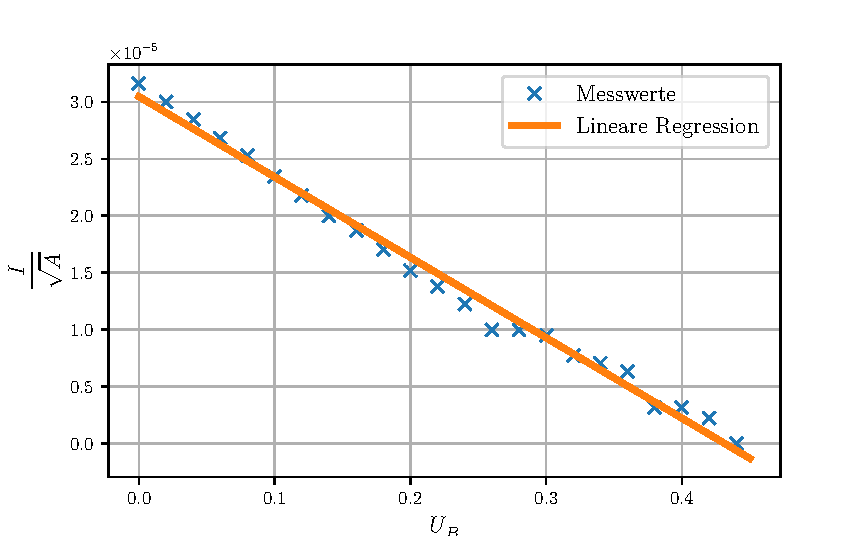
\includegraphics{plot2.pdf}
  \caption{Magnetfeldstärke bei verschiedenen Abständen $x$ zum Mittelpunkt bei einem 
  Spulenabstand von $a=12 \, \unit{\cm}$.}
  \label{fig:Helm12}
\end{figure}

\begin{figure}
  \centering
  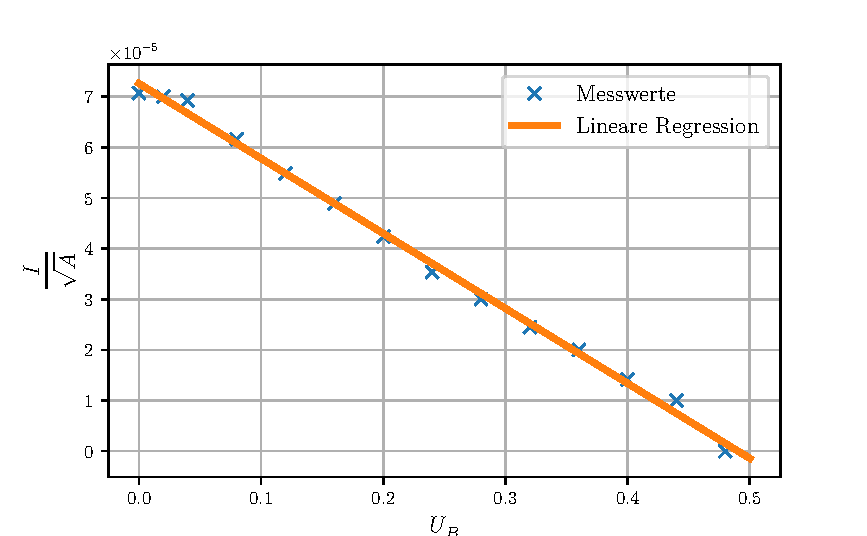
\includegraphics{plot3.pdf}
  \caption{Magnetfeldstärke bei verschiedenen Abständen $x$ zum Mittelpunkt bei einem 
  Spulenabstand von $a=14 \, \unit{\cm}$}
  \label{fig:Helm14}
\end{figure}

\begin{figure}
  \centering
  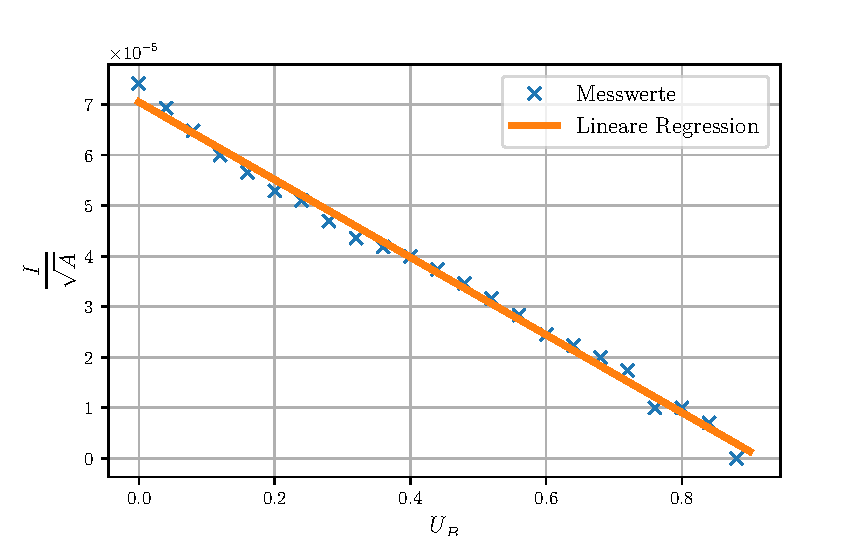
\includegraphics{plot4.pdf}
  \caption{Magnetfeldstärke bei verschiedenen Abständen $x$ zum Mittelpunkt bei einem 
  Spulenabstand von $a=16 \, \unit{\cm}$}
  \label{fig:Helm16}
\end{figure}

Es wird die prozentuelle Abweichung der Theoriekurve zu den Messwerten bei $x=0$ berechnet.
Für $a=12 \, \unit{\cm}$ ergibt das 11,24 \%, für $a=14 \, \unit{\cm}$ 13,26 \% und für $a=16 \, \unit{\cm}$ 15,67 \%.\\
Für die gezeigte Theoriekurven wurde die Superposition von \autoref{eqn:ringspule} ausgenutzt, da es sich
bei dem Helmholtz-Spulenpaar um zwei Ringspulen handelt.\\

\subsection{Hysteresekurve}

Bei dieser Versuschsreihe wird das Magnetfeld einer Ringspule mit Luftspalt mithilfe einer
transversalen Hall-Sonde gemessen. Die Ringspule hat $n=595$ Windungen und einen Radius von $r_T=13,5 \, \unit{\cm}$. \\
Es wird eine beliebige Spannung verwendet. Zunächst wird 
die bleibende Remanenz der Ringspule möglichst neutralisiert und dann der Strom bis 10 A
hochgeregelt. Dabei wird das Magnetfeld gemessen.\\
Danach wird der Strom wieder runtergeregelt, es wird umgepolt und erneut auf 10 A erhöht.
Erneut wird der Strom wieder bis auf Null runtergeregelt, ein letztes Mam umgepolt und der Strom
wieder bis auf 10 A erhöht.\\
Um die Hysteresekurve zu zeichnen, wird zunächst die Feldstärke $H$ ausgerechnet. Zur Berechnung verwendet wir \autoref{eqn:H}.


\begin{table}
  \centering
  \caption{Messwerte des Magnetfelds in der Ringspule.}
  \label{tab:Hysterese}
  \begin{tabular}{c c c}
    \toprule
    $B/\unit{\tesla} \cdot 10^{-3}$ & $I/\unit{\ampere}$ & $H/\unit{\ampere}/\unit{\m}$ \\
    \midrule
    -2.8  &  0 &  0        \\
    111.5 &  1 &  701.8    \\
    280.8 &  2 &  1403.6   \\
    400.0 &  3 &  2105.4   \\
    479.8 &  4 &  2807.3   \\
    538.3 &  5 &  3509.1   \\
    581.6 &  6 &  4210.9   \\
    620.1 &  7 &  4912.7   \\
    648.0 &  8 &  5614.5   \\
    677.3 &  9 &  6316.3   \\
    704.3 &  10 & 7018.2   \\
    685.4 &  9   &    6316.3   \\
    674.5 &  8   &    5614.5   \\
    653.3 &  7   &    4912.7   \\
    630.7 &  6   &    4210.9   \\
    592.4 &  5   &    3509.1   \\
    571.0 &  4   &    2807.3   \\
    525.0 &  3   &    2105.4   \\
    461.3 &  2   &    1403.6   \\
    343.0 &  1   &    701.8    \\
    129.0 &  0   &    0        \\
    -78.1 &  -1   &   -701.8   \\
    -251.1 & -2   &   -1403.6  \\
    -395.8 & -3   &   -2105.4  \\
    -480.0 & -4   &   -2807.3  \\
    -541.7 & -5   &   -3509.1  \\
    -586.4 & -6   &   -4210.9  \\
    -626.7 & -7   &   -4912.7  \\
    -657.0 & -8   &   -5614.5  \\
    -685.5 & -9   &   -6316.3  \\
    -713.2 & -10  &   -7018.2  \\
    -696.8 &  -9  &   -6316.3  \\
    -678.9 &  -8  &   -5614.5  \\
    -660.2 &  -7  &   -4912.7  \\
    -637.1 &  -6  &   -4210.9  \\
    -607.1 &  -5  &   -3509.1  \\
    -573.1 &  -4  &   -2807.3  \\
    -527.0 &  -3  &   -2105.4  \\
    -463.2 &  -2  &   -1403.6  \\
    -330.3 &  -1  &   -701.8   \\
    \bottomrule
  \end{tabular}
\end{table}


\begin{table}
  \centering

  \begin{tabular}{c c c}
    \toprule
    
    \midrule
    -123.6 &  0   &   0        \\
    77.8   &  1   &   701.8    \\
    257.5  & 2    &   1403.6   \\
    391.9  & 3    &   2105.4   \\
    484.0  & 4    &   2807.3   \\
    542.8  & 5    &   3509.1   \\
    591.1  & 6    &   4210.9   \\
    626.8  & 7    &   4912.7   \\
    658.3  & 8    &   5614.5   \\
    686.2  & 9    &   6316.3   \\
    718.9  & 10   &   7018.2   \\
    \bottomrule
  \end{tabular}
\end{table}


\begin{figure}
  \centering
  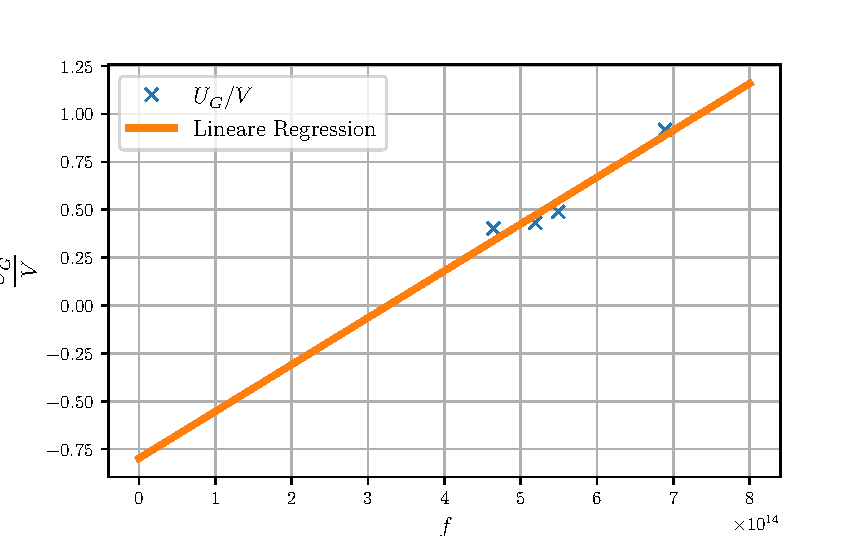
\includegraphics{plot5.pdf}
  \caption{Hysteresekurve der Ringspule.}
  \label{fig:Hysterese}
\end{figure}

Anhand der Hysteresekurve lassen sich eine Sättigungsmagnetisierung von $B_s = 718 \cdot 10^{-3} \, \unit{\tesla}$,
eine Koerzitivkraft von $H_c = -370 \, \unit{\ampere}/\unit{\m}$ und eine Remanenz von $B_r= 129 \cdot 10^{-3} \, \unit{\tesla}$.\\
